\subsection*{3.4\quad 深度学习基础}
\subsubsection*{3.4.1\quad 深度学习与表示学习}

\noindent 在开始学习深度学习之前,先要澄清一个常见的误解:很多人把深度学习、监督学习、强化学习当作同一层级的概念来理解,仿佛它们是几种互相并列的学习方法。这种理解并不准确。更精确地说,前面3.3节讨论的监督学习、无监督学习、强化学习描述的是学习问题如何被设定,即训练信号从哪里来、学习目标如何定义;而深度学习描述的是用什么样的函数族去表示规律,以及用什么方式去训练这个函数族。用更通俗的话讲,监督学习意味着这道题带有可对照的目标,无监督或自监督强调从数据自身构造学习信号,强化学习则通过与环境交互、尝试与错误来改进行为策略;至于完成这些任务所使用的"模型工具箱",既可以是简单的线性模型,也可以是复杂的深度网络。把深度学习放到"模型与表示"的维度来理解,读者就不会把它与监督学习或强化学习误认为同一层级的概念。

\noindent 从更抽象的角度看,深度学习的核心计算结构是多层可微函数的复合:把许多相对简单的变换按层串联,每一层对上一层的输出再做一次变换,最终得到任务所需的输出。具体来说,给定输入 $x$,一个 $L$ 层网络的前向计算可以写成
\[ h^{(0)}=x,\qquad h^{(\ell)}=f_\ell\!\left(h^{(\ell-1)};\theta_\ell\right)\ \ (\ell=1,\dots,L),\qquad \hat y=h^{(L)}. \]
其中 $h^{(\ell)}$ 是第 $\ell$ 层的中间表示,$\theta_\ell$ 是该层参数,整体参数记为 $\theta=\{\theta_\ell\}_{\ell=1}^L$。把这些层串起来,就得到整体函数
\[ \hat y=f(x;\theta)=f_L\!\left(\cdots f_2(f_1(x;\theta_1);\theta_2)\cdots;\theta_L\right). \]
这组表达式的意义并不在于"网络一定长这样",而在于强调深度网络是一种分层表示的计算框架:每一层把上一层的表示变换成新的表示,使得表示在层间逐步发生抽象与重组。早期层通常更贴近原始输入形式,后期层逐步变得更抽象、更贴近任务目标。深度学习之所以常与"表示学习"绑定讨论,正是因为它并不只学习一个最终输出规则,而是把中间表示本身也作为学习对象,通过数据驱动的方式自动形成对任务有用的特征结构。

\medskip
\noindent \begin{figure}[htbp]
\centering
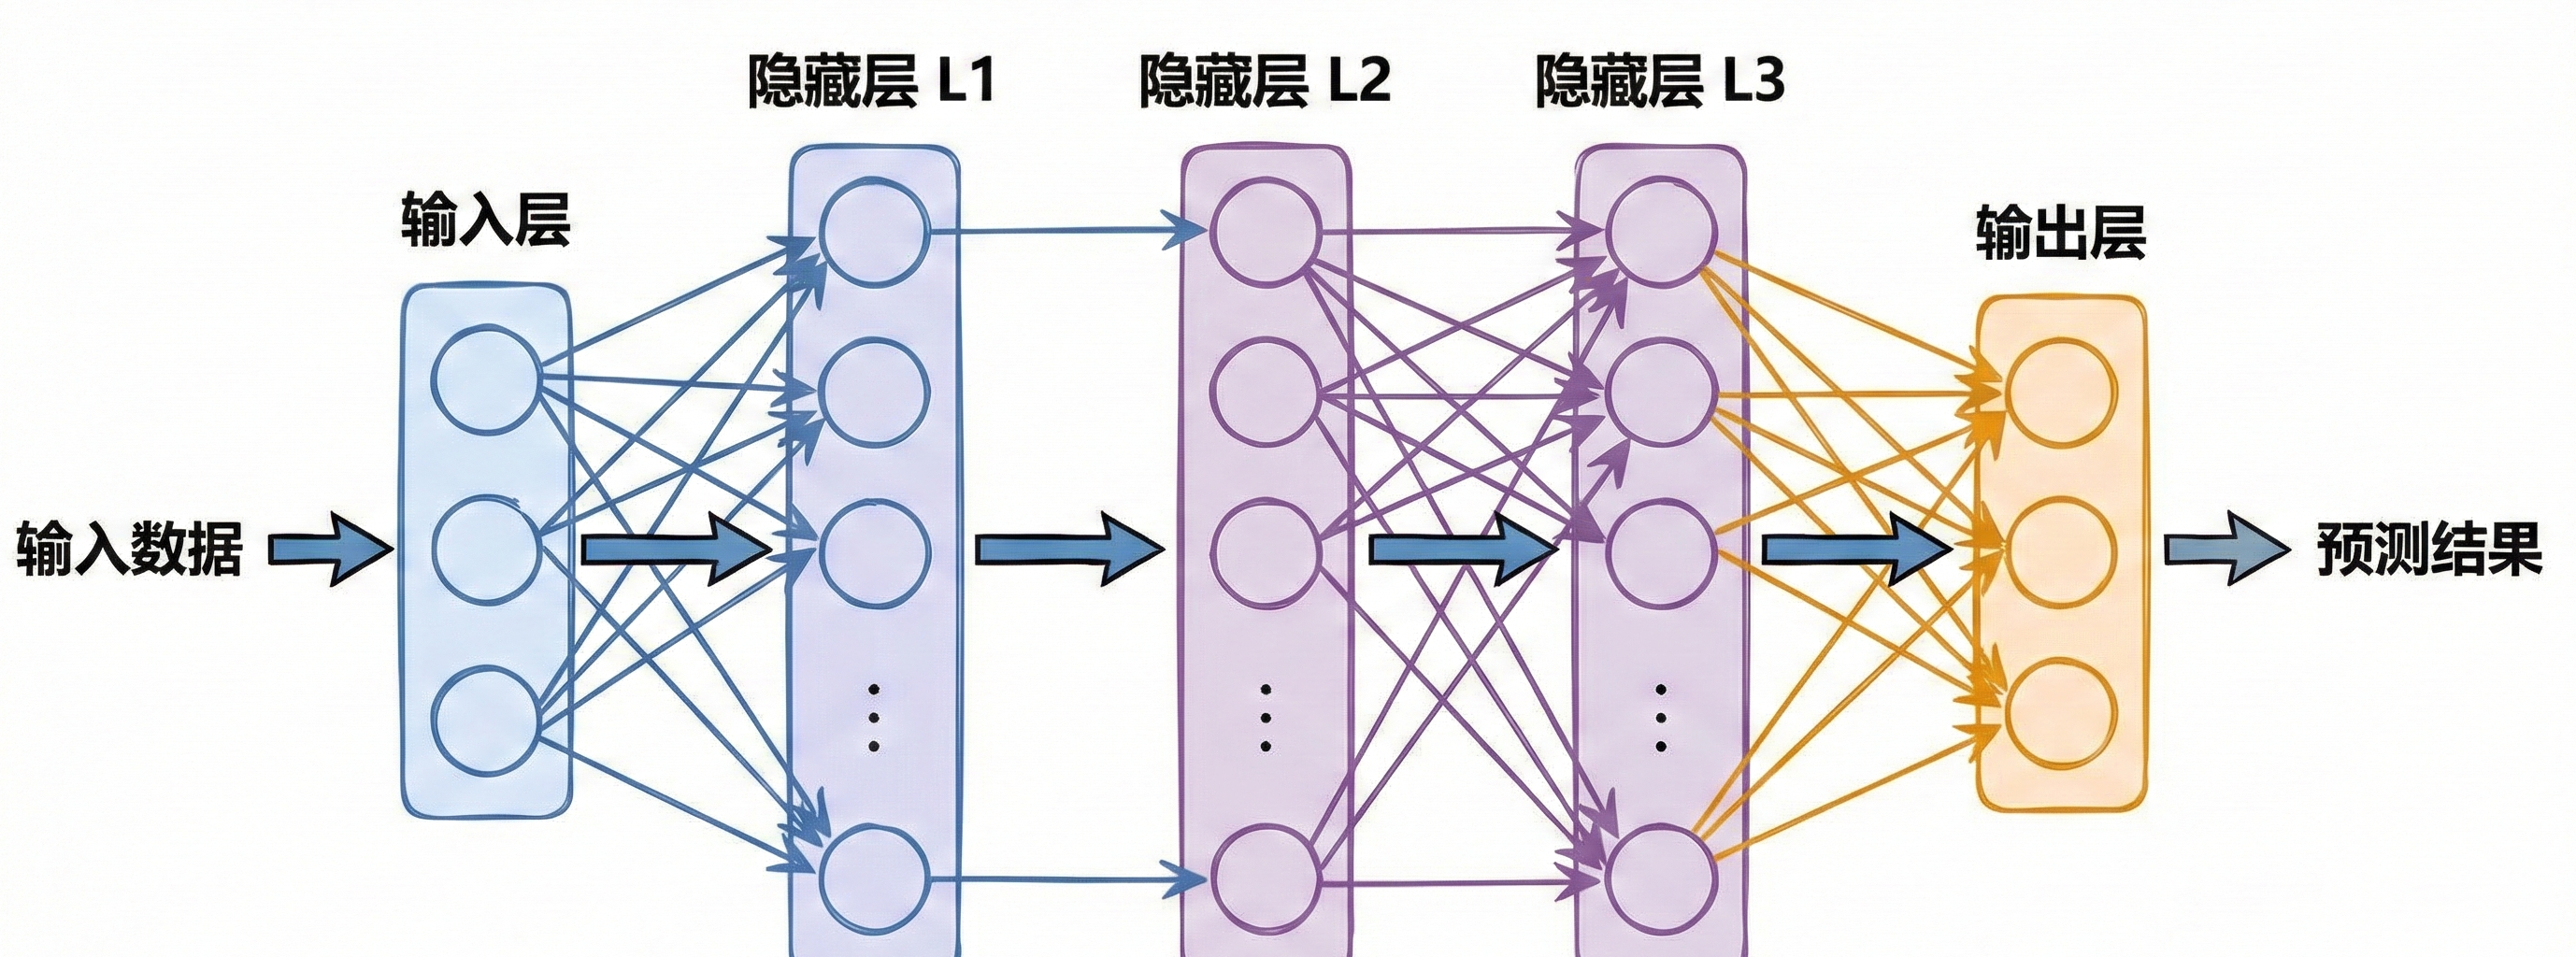
\includegraphics[width=0.75\textwidth]{figures/fig-3-4-1-deep-network-architecture.png}
\caption{\textbf{深度网络分层结构示意图}}
\label{fig:3-4-1-deep-network-architecture}
\end{figure}

\noindent 以图像识别为例。输入是一张照片时,靠近输入的层往往首先捕捉局部的边缘、纹理等低层模式;随着层数加深,这些低层模式会被逐步组合为更稳定的局部结构,再进一步组合为更高层的语义部件,最终形成对"物体类别"等任务目标更直接的表示。可以把它类比为人类的视觉理解过程:先看到线条和色块,再看出形状,最后形成对整体对象的判断。深度网络的分层结构提供了一种可计算的机制,使这种"从局部到整体、从具体到抽象"的表征转化能够在数据上被学习出来,而不是由人预先规定。

\noindent 这也解释了深度学习与传统特征工程路径的关键差异。传统做法往往把"特征提取"与"任务学习"拆成两个阶段:先由人设计特征,再用相对简单的模型去拟合。例如识别农作物是否患病时,可能先手工构造颜色分布、病斑大小数量等特征,再用逻辑回归或支持向量机分类。深度学习把这两件事合并为一个端到端的过程:特征表示与任务目标由同一个损失函数驱动,并通过同一次训练共同得到。换句话说,深度学习的关键不在于层数多本身,而在于它用统一的目标函数与梯度优化,让模型能够在任务约束下自动形成有用的中间表示,从而减少对人工指定"应该看什么特征"的依赖。

\medskip
\noindent \begin{figure}[htbp]
\centering
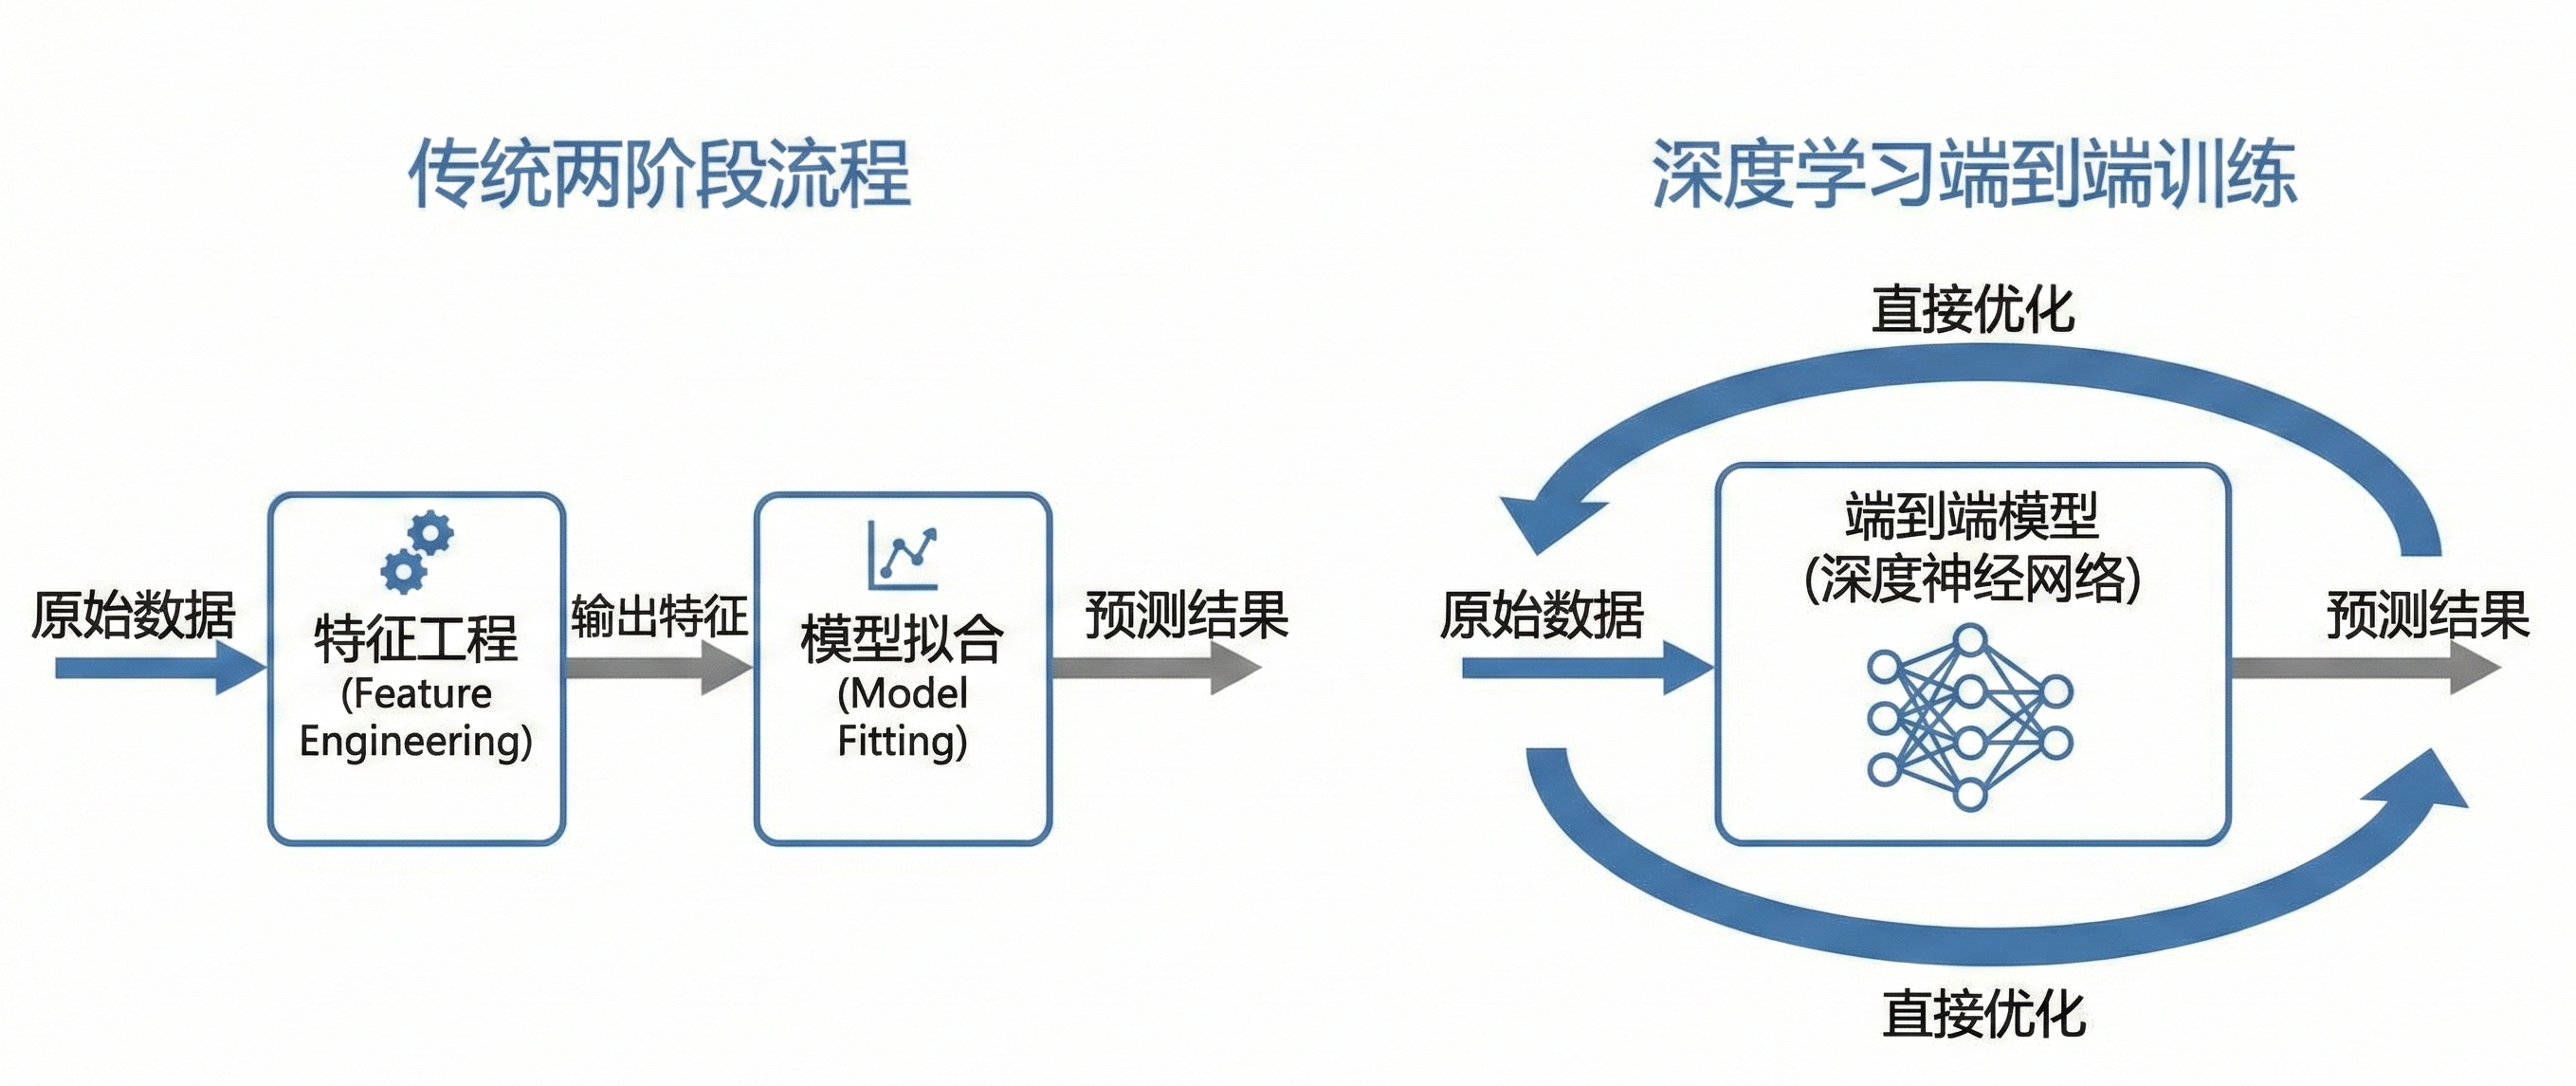
\includegraphics[width=0.75\textwidth]{figures/fig-3-4-2-end-to-end-training.png}
\caption{\textbf{端到端训练与传统两阶段流程对比示意图}}
\label{fig:3-4-2-end-to-end-training}
\end{figure}

\noindent 从训练目标的形式看,深度学习通常同样被写成一个优化问题。以最常见的监督学习为例,给定数据集 $\mathcal D=\{(x_i,y_i)\}_{i=1}^n$,选择损失函数 $L(\cdot,\cdot)$ 来衡量预测 $\hat y_i=f(x_i;\theta)$ 与真实 $y_i$ 的偏差,训练目标是最小化平均损失,并常加入正则项控制复杂度:
\[ \min_{\theta}\; J(\theta)=\frac{1}{n}\sum_{i=1}^n L\big(y_i,f(x_i;\theta)\big)+\lambda\,\Omega(\theta). \]
这一形式与前面3.3节的监督学习在结构上完全一致,差别主要在于此处的 $f(x;\theta)$ 是由多层复合构成的高容量函数族。正因为容量高,深度网络能够拟合更复杂的输入—输出关系,但也更依赖合理的训练策略与泛化控制,否则容易出现训练不稳定或过拟合。深度"为何重要",也可以在这一框架下被理解:一方面,多层复合通常带来更强的表达效率,许多复杂映射若用单层或浅层模型表达,往往需要大量参数,而用多层结构可以通过逐层组合,以更紧凑的方式实现同样的函数;另一方面,许多现实数据具有天然的层级生成或组合结构,例如视觉中的边缘—形状—部件—物体,语言中的词—短语—句法—语义,分层表示为模型提供了更合适的归纳偏好,使其更容易以可复用的组件组织复杂规律。

\noindent 需要注意的是,表达能力强并不自动意味着训练就容易。深度网络训练依赖梯度法,通过反向传播高效计算 $\nabla_\theta J(\theta)$,再用梯度下降或其变体更新参数
\[ \theta\leftarrow \theta-\eta \nabla_\theta J(\theta), \]
其中 $\eta$ 是学习率。对读者而言,此处需要抓住一个核心事实:深度学习并没有绕开传统学习理论的基本约束,它只是把可表示的函数空间扩展得更大,并通过可微分计算图与梯度优化使大规模参数学习成为可能。后续常见的训练技巧(初始化、归一化、正则化、优化器、数据增强等)都可以理解为在这个高容量、强非线性的函数空间里,让梯度优化更稳定,让学到的表示更可泛化。理解了深度学习的这一定位之后,读者就能够在后续章节更自然地接受卷积神经网络、Transformer等具体结构:它们是在同一深度学习框架下,为不同数据形态引入不同的结构偏好与计算方式,从而更高效地学习有用的表示。
\subsubsection*{3.4.2\quad 前向计算与训练机制}

\noindent 深度学习最需要把握的,不是某一种网络结构的细节,而是一套稳定的计算与训练闭环:网络如何把输入变成输出,训练又如何把输出与目标之间的差距反过来变成参数更新。只要这条闭环清晰,后面无论遇到卷积神经网络还是Transformer,都可以把它们看作是在同一训练机制下更换了不同的前向计算模块。实践中的训练过程可以概括为四个环节的循环往复:前向计算把输入映射为输出;损失函数把输出与真实标签之间的差距量化为一个标量;反向传播把这个差距分解为对各层参数的梯度信号;优化器再依据梯度更新参数。训练轮次不断推进,直到性能不再提升或达到预定的停止条件。

\noindent 神经网络的前向计算通常可以概括为线性变换与非线性变换的交替复合。设输入为 $x\in\mathbb R^{d_0}$,记 $h^{(0)}=x$,第 $\ell$ 层的线性部分为
\[ z^{(\ell)} = W^{(\ell)}h^{(\ell-1)} + b^{(\ell)},\]
其中 $W^{(\ell)}\in\mathbb R^{d_\ell\times d_{\ell-1}}$ 是权重矩阵,$b^{(\ell)}\in\mathbb R^{d_\ell}$ 是偏置向量;随后通过激活函数得到
\[ h^{(\ell)}=\phi\!\left(z^{(\ell)}\right).\]
把这些层按顺序串起来,就得到一个整体复合函数 $f(x;\theta)$,其中参数 $\theta=\{W^{(\ell)},b^{(\ell)}\}_{\ell=1}^L$。直观上,这相当于把输入逐层重编码:前几层往往形成更局部、更简单的模式,中间层把这些模式组合成更抽象的表示,最后一层把抽象表示映射为任务需要的输出。以识别农作物病害为例,靠近输入的层可能先对叶片的颜色与纹理敏感;更深的层逐步形成对病斑形状、边界与分布模式的表征;最终输出层将这些表征汇聚为对病害类型及严重程度的判断。

\medskip
\noindent \begin{figure}[htbp]
\centering
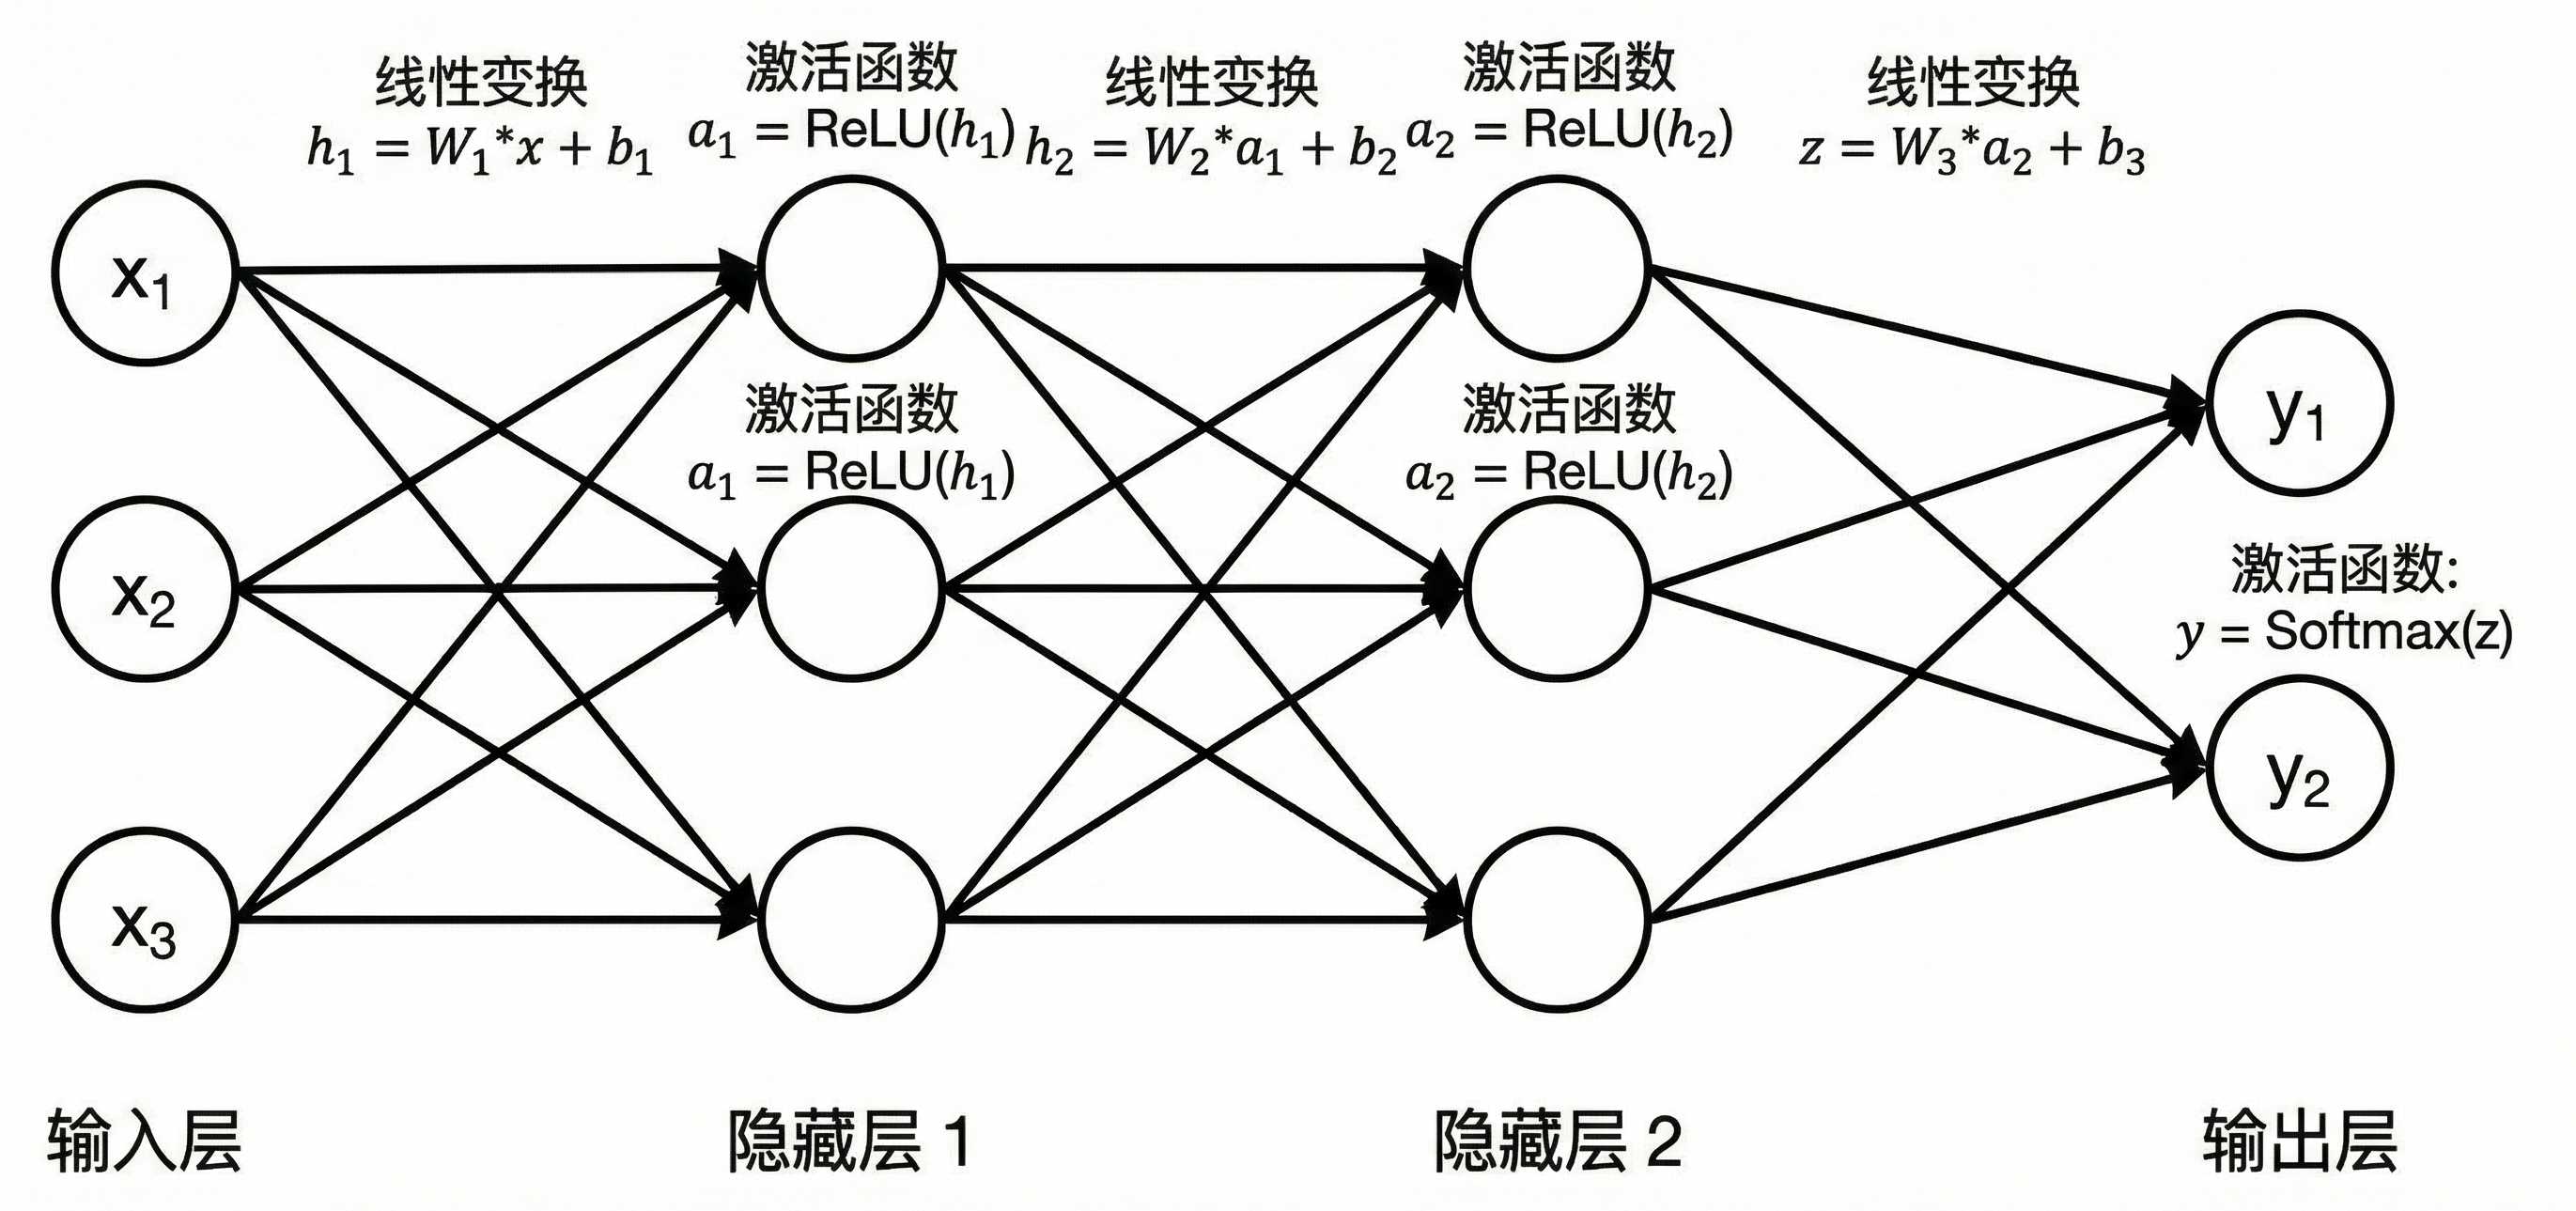
\includegraphics[width=0.75\textwidth]{figures/fig-3-4-3-forward-propagation.png}
\caption{\textbf{神经网络前向计算示意图}}
\label{fig:3-4-3-forward-propagation}
\end{figure}

\noindent 这种"线性变换堆叠很多层"的结构之所以能够表达复杂规律,关键在于非线性激活的引入。如果把所有激活函数 $\phi$ 都去掉,那么多层线性变换的复合仍然等价于一次线性变换,网络再深也只能表达线性关系。非线性提供了"弯折空间",使网络能够表示复杂的非线性函数与非线性决策边界。可以用一个近似的几何类比来理解:如果真实关系是弯曲的,只允许用直线去拟合往往无法贴合;但若允许用多段折线逐段逼近,就可以通过不断增加折点来逼近任意复杂的曲线。激活函数的作用,就是让每一层都有产生一次"折点/弯折"的能力,多层叠加便形成更强的表示能力。常见激活函数包括 ReLU、tanh、sigmoid 等;在训练机制的层面,重要的不是它们的具体形状细节,而是它们使网络从线性模型跃迁为非线性模型。ReLU 之所以最常用,一个直接原因是其形式简单、计算高效,并且在大规模训练中表现稳定。

\noindent 前向计算的最后一步还需要与任务类型对齐,以保证网络输出的语义与训练目标一致。回归问题往往直接输出实数向量 $\hat y$;二分类问题通常输出一个概率 $\hat p\in(0,1)$;多分类问题则输出对各类别的概率分布。对应地,输出层常写为
\[ \hat y = g\!\left(W^{(L)}h^{(L-1)}+b^{(L)}\right),\]
其中 $g$ 的选择取决于任务。二分类常用 sigmoid:
\[ \hat p=\sigma(z)=\frac{1}{1+e^{-z}},\]
多分类常用 softmax:
\[ \hat p_k=\frac{e^{z_k}}{\sum_{j=1}^K e^{z_j}}.\]
把输出解释为概率的意义在于,训练目标可以自然地写成"让真实标签在模型输出分布下尽可能大",从而得到对数似然与交叉熵等标准形式,使训练过程具有清晰的统计解释与可比较的评价尺度。

\noindent 有了与任务对齐的输出语义,训练目标就可以被明确地写成一个优化问题。给定样本 $(x_i,y_i)$,网络前向得到预测 $\hat y_i=f(x_i;\theta)$,损失函数 $L(y_i,\hat y_i)$ 衡量预测与真实的差异。训练的目标是最小化训练集上的平均损失,必要时加入正则项以控制复杂度:
\[ J(\theta)=\frac{1}{n}\sum_{i=1}^n L\big(y_i,f(x_i;\theta)\big)+\lambda\Omega(\theta),\qquad \theta^\ast=\arg\min_\theta J(\theta).\]
在这一步上,监督学习与深度学习并没有本质差异:差异主要来自 $f(\cdot;\theta)$ 的函数族更复杂、参数更多、表达能力更强,因此既能拟合更丰富的模式,也更需要稳定的训练策略与有效的泛化控制。

\noindent 真正让深度网络可训练的是反向传播与基于梯度的优化。反向传播并不是另一套独立的学习规则,它只是把链式法则系统化地应用到计算图上,用高效的方式计算出 $\nabla_\theta J(\theta)$。一次参数更新可以写成
\[ \theta \leftarrow \theta-\eta \nabla_\theta J(\theta),\]
其中 $\eta$ 是学习率。直观地理解,前向计算告诉我们网络当前输出什么、偏差在哪里;反向传播告诉我们这些偏差应当分别归因到哪些参数上,以及每个参数沿哪个方向微调最能让损失下降。梯度就是这种"应该怎么改"的定量化信号。为了把反向传播在"传什么"说清楚,可以用误差信号的传播来描述。对第 $\ell$ 层,定义该层线性输出 $z^{(\ell)}$ 上的误差信号
\[ \delta^{(\ell)}=\frac{\partial J}{\partial z^{(\ell)}}.\]
则参数梯度满足
\[ \frac{\partial J}{\partial W^{(\ell)}}=\delta^{(\ell)}(h^{(\ell-1)})^\top,\qquad \frac{\partial J}{\partial b^{(\ell)}}=\delta^{(\ell)},\]
而误差信号在层与层之间的传播满足
\[ \delta^{(\ell)}=\big((W^{(\ell+1)})^\top \delta^{(\ell+1)}\big)\odot \phi'\!\left(z^{(\ell)}\right),\]
其中 $\odot$ 表示按元素相乘。这个关系式表达的含义很直接:上一层的误差来自下一层误差的回传,再乘上本层激活函数在当前位置的导数,刻画"本层输出的微小变化会对整体损失造成多大影响"。反向传播之所以高效,是因为它把整网的梯度计算分解为局部的矩阵运算,并复用前向阶段缓存的中间量,避免了对同一子表达式的重复求导与重复计算。

\medskip
\noindent \begin{figure}[htbp]
\centering
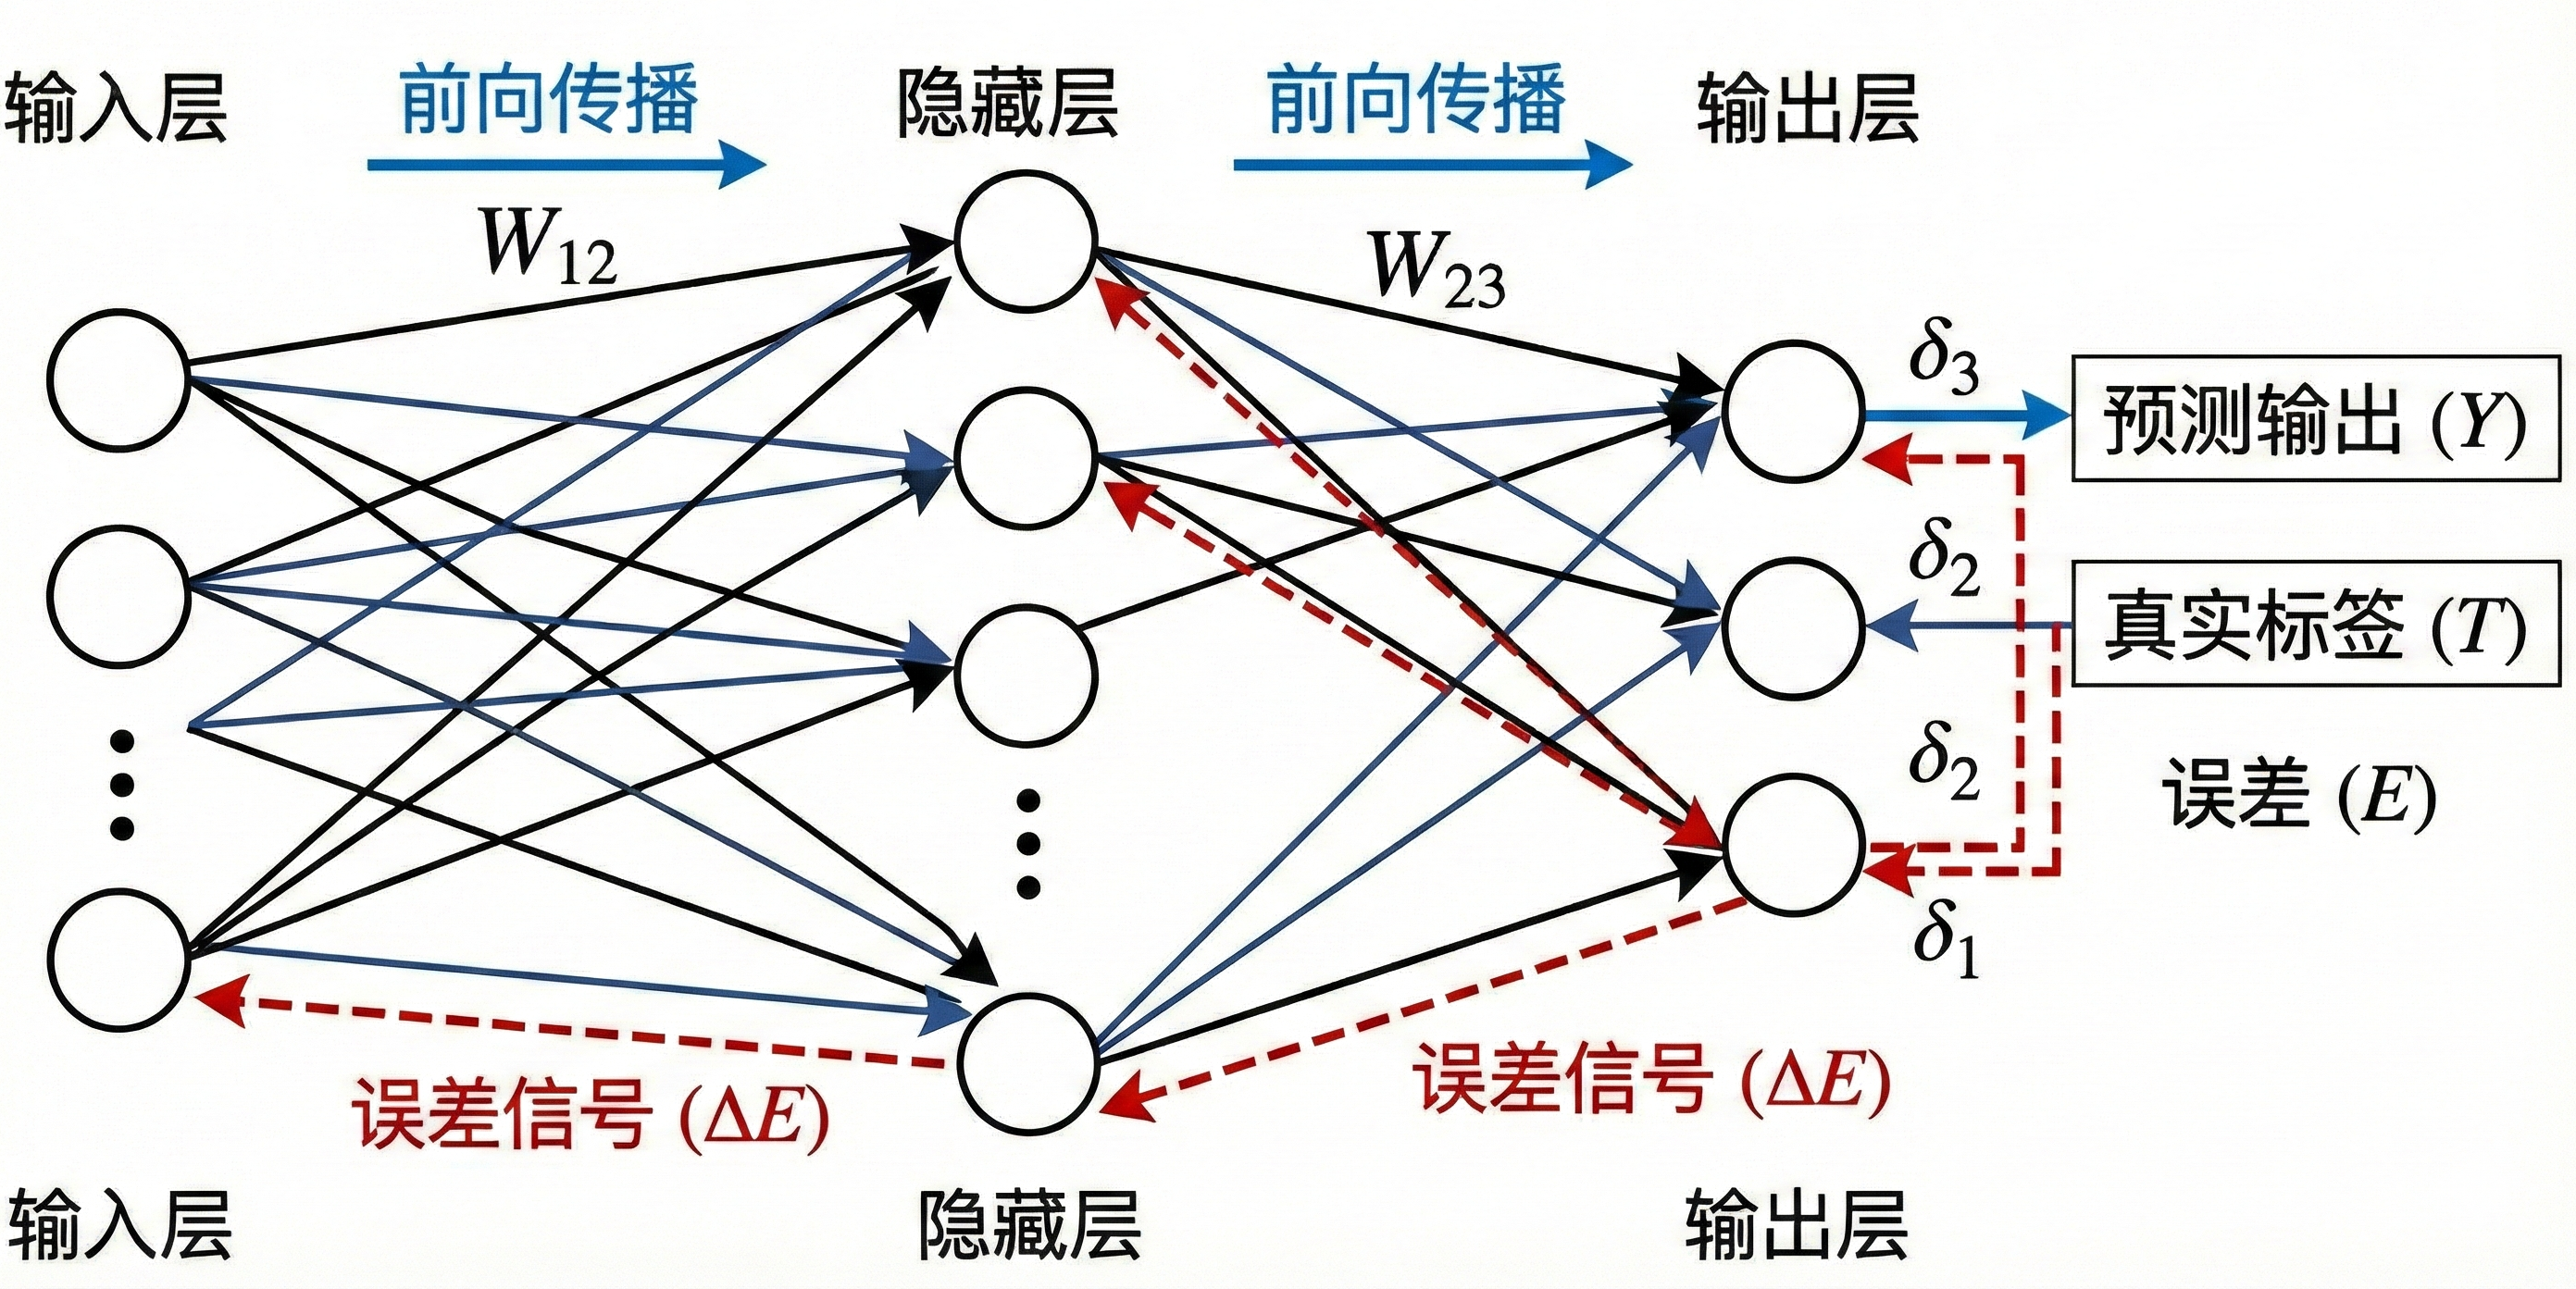
\includegraphics[width=0.75\textwidth]{figures/fig-3-4-4-backpropagation.png}
\caption{\textbf{反向传播误差信号回传示意图}}
\label{fig:3-4-4-backpropagation}
\end{figure}

\noindent 在工程实践中,很少使用全量梯度下降,而更常用小批量随机梯度下降:将数据划分为批次 $B$,每次用一个批次近似整体梯度
\[ \nabla_\theta J(\theta)\approx \frac{1}{|B|}\sum_{i\in B}\nabla_\theta L\big(y_i,f(x_i;\theta)\big),\]
然后执行一次参数更新。这样做一方面显著提高计算效率,使训练可以在有限显存与时间预算下推进;另一方面,批次梯度所带来的随机噪声在一定程度上反而有助于优化过程跳出不佳的局部区域或平坦区域,从而更容易获得更好的解。优化器可以是基础的随机梯度下降,也可以加入动量或自适应学习率机制(如 Adam)以改善收敛速度与稳定性,但在训练机制的层面,它们做的仍是同一件事:利用梯度信息确定更新方向,并用不同的规则调节更新幅度、平滑噪声与控制训练动态。

\noindent 归纳起来,网络结构改变的是前向计算的具体形式与所引入的归纳偏置;但"前向—损失—反向—更新"的训练闭环保持不变。理解这一点,读者在后续学习卷积神经网络的卷积算子或 Transformer 的注意力算子时,关注点就会自然落在:新的前向模块如何改变信息的流动与表示的组织方式,而不是误以为需要重新学习一套完全不同的训练逻辑。
\subsubsection*{3.4.3\quad 卷积神经网络基础}

\noindent 卷积神经网络之所以适合处理图像,并不因为它采用了与其他神经网络完全不同的训练机制。它同样遵循前向计算、损失函数、反向传播、梯度更新的训练闭环。卷积神经网络的关键变化发生在前向计算的结构设计上:它把"局部模式可以在整幅图上反复出现"这一经验写进网络结构,使网络在学习时天然倾向于提取边缘、角点、纹理等局部结构,并把这些结构在空间上的分布以特征图的形式保留下来。图\ref{fig:cnn-sliding-window}给出了一个更贴近"卷积在做什么"的示意:左侧输入图像存在明显的明暗分界;中间展示卷积核在输入上以滑动窗口方式做局部点积(滑动窗口 \& 点积);图中用两组方向性边缘检测核(示例为 Sobel $X$ 与 Sobel $Y$)分别对输入做卷积,从而得到两张输出特征图。可以看到,其中一张特征图在分界处出现高亮响应带,说明该方向的卷积核与图像中的边缘方向匹配;另一张特征图整体接近零,说明在该输入下,与其对应方向的边缘并不明显。右侧进一步把两个方向的边缘响应进行融合,得到更稳定的边缘表征。

\begin{figure}[htbp]
\centering
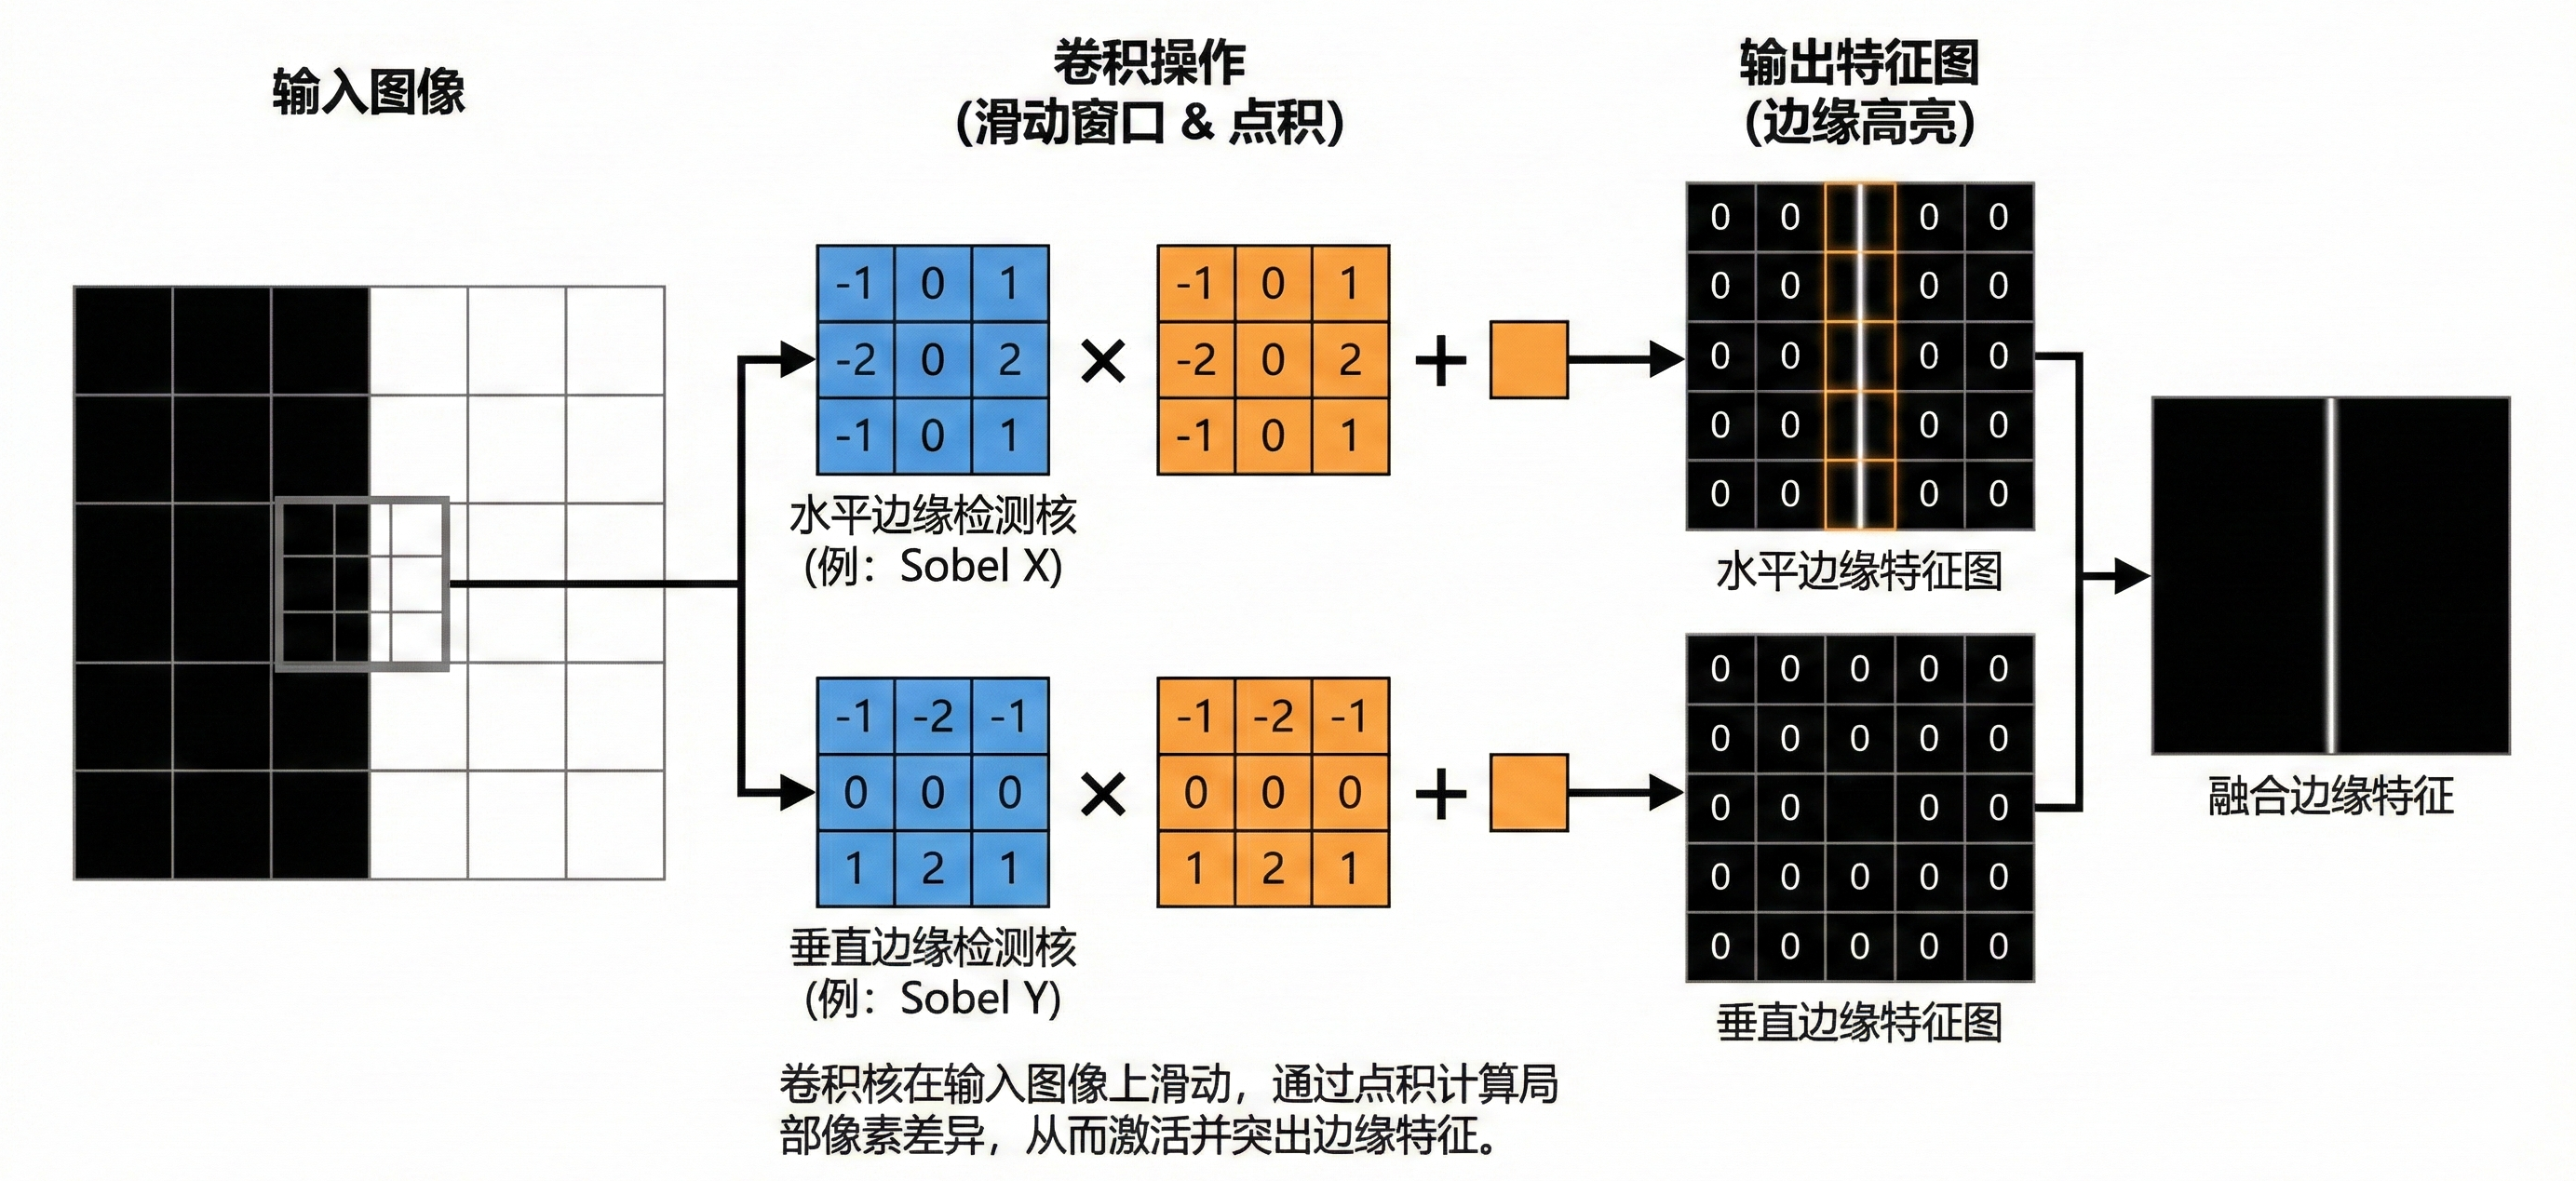
\includegraphics[width=0.9\textwidth]{figures/fig-cnn-sliding-window}
\caption{卷积用于边缘检测的直观示意:卷积核在输入图像上滑动,在每个局部窗口内做点积得到响应;使用两组方向性边缘检测核(示例为 Sobel $X$ 与 Sobel $Y$)可分别产生两张方向特征图,其中与输入边界方向一致的特征图在边界处出现高亮响应带;将两张方向特征图融合可得到更完整的边缘特征。}
\label{fig:cnn-sliding-window}
\end{figure}

\noindent 在最常见的二维情形中,输入是一张二维网格(例如灰度图像)$X\in\mathbb R^{H\times W}$。卷积层用一个小的权重矩阵(卷积核)$W\in\mathbb R^{k\times k}$在输入上滑动。每次滑动,卷积核只覆盖输入图像的一块局部区域,并在该局部窗口上做加权求和,得到输出特征图 $Y\in\mathbb R^{(H-k+1)\times(W-k+1)}$:
\[ Y_{i,j}=\sum_{u=0}^{k-1}\sum_{v=0}^{k-1}W_{u,v}\,X_{i+u,\,j+v}+b,\]
其中 $b$ 是偏置项。随后通常还会接一个非线性激活函数 $\phi(\cdot)$ 得到
\[ H_{i,j}=\phi(Y_{i,j}).\]
若输入是多通道(例如 RGB 图像),则 $X\in\mathbb R^{H\times W\times C}$。此时卷积核在空间维度仍是 $k\times k$,但同时覆盖 $C$ 个通道,输出每个位置的值来自对所有通道对应局部窗口的加权汇总;多个卷积核会产生多个输出通道,从而形成更丰富的特征表示。就本节的目的而言,理解单通道卷积的核心计算与"滑动窗口点积产生特征图"的含义,已足以把握卷积神经网络的基本思想。

\noindent 卷积计算的直观意义,可以直接借助图\ref{fig:cnn-sliding-window}中"方向性边缘检测核"的对比来理解。图中给出两组 $3\times3$ 的边缘检测核(示例为 Sobel $X$ 与 Sobel $Y$),它们的系数结构体现了"对某一方向的像素差异更敏感"的偏好:当卷积核覆盖的局部窗口跨越明暗分界时,窗口两侧像素值差异显著,点积结果会出现较大的幅度,从而在输出特征图的对应位置形成高亮响应;当局部窗口落在灰度相对均匀的区域时,加权求和相互抵消,输出更接近零。因此,在图\ref{fig:cnn-sliding-window}中,与输入边界方向相匹配的那一路卷积会在分界处产生一条明显的高亮带,而另一方向由于缺乏对应的边缘结构,响应整体较弱。进一步地,将两路方向响应进行融合,可以得到更完整、更鲁棒的边缘表征,这也是实践中常见的做法:先用不同卷积核提取互补的局部结构,再在后续层中把这些结构组合成更高层次的形状与语义。

\noindent 从结构角度看,卷积层的优势可以概括为"用局部计算生成空间化表示"。每一个输出位置只由输入的一小块区域决定,这一小块区域称为感受野。对上式而言,$Y_{i,j}$ 只依赖 $X$ 的一个 $k\times k$ 子矩阵;这正对应图\ref{fig:cnn-sliding-window}中以滑动窗口标出的局部点积过程。局部计算来自对图像数据的基本判断:边缘是局部灰度突变,纹理是局部重复模式,角点是局部方向变化。与其让网络在第一层就把整张图像的所有像素一次性混合,不如先在局部范围内检测可复用的小模式,再逐层把这些小模式组合成更大的结构。局部连接还会显著降低参数规模:若用全连接层把 $H\times W$ 个像素直接映射到 $m$ 个隐藏单元,参数量是 $mHW$ 量级;而卷积层对单个卷积核只需要 $k^2$ 个参数(多通道时为 $k^2C$),从而更容易在有限数据下学习到可泛化的局部规律。

\noindent 为了把卷积的"滑动窗口加权求和"落到可计算的步骤上,可以给出一个可手算的最小例子。考虑一个 $3\times3$ 的输入矩阵
\[ X=\begin{pmatrix} 1&2&0\\ 0&1&3\\ 2&1&1 \end{pmatrix},\]
取一个 $2\times2$ 卷积核
\[ W=\begin{pmatrix} 1&0\\ 0&-1 \end{pmatrix},\quad b=0.\]
采用步幅 $1$、无填充,则输出 $Y$ 为 $2\times2$。逐位置计算:左上角窗口为 $\begin{pmatrix}1&2\\0&1\end{pmatrix}$,因此
\[ Y_{0,0}=1\cdot 1+0\cdot 2+0\cdot 0+(-1)\cdot 1=0;\]
右上角窗口为 $\begin{pmatrix}2&0\\1&3\end{pmatrix}$,因此
\[ Y_{0,1}=1\cdot 2+0\cdot 0+0\cdot 1+(-1)\cdot 3=-1;\]
左下角窗口为 $\begin{pmatrix}0&1\\2&1\end{pmatrix}$,因此
\[ Y_{1,0}=1\cdot 0+0\cdot 1+0\cdot 2+(-1)\cdot 1=-1;\]
右下角窗口为 $\begin{pmatrix}1&3\\1&1\end{pmatrix}$,因此
\[ Y_{1,1}=1\cdot 1+0\cdot 3+0\cdot 1+(-1)\cdot 1=0.\]
汇总得到
\[ Y=\begin{pmatrix} 0&-1\\ -1&0 \end{pmatrix}.\]
如果再接一个 ReLU 激活 $\phi(t)=\max(0,t)$,则负响应会被截断为 0。这个例子的目的不是追求某个任务的"正确输出",而是让读者明确:卷积层输出的每一个位置,本质上就是卷积核在对应局部窗口上的一次点积与加权求和;当滑动窗口跨越某类局部结构(例如明暗分界或特定方向的梯度变化)时,卷积核会产生显著响应,并把这种响应以"特征图上的高值区域"标注出来。图\ref{fig:cnn-sliding-window}中的边缘高亮带,正是这种局部响应在方向性边缘检测核与含边界输入这一组合下的直观呈现。
\subsubsection*{3.4.4\quad Transformer 基础}

\medskip
\begin{figure}[htbp]
\centering
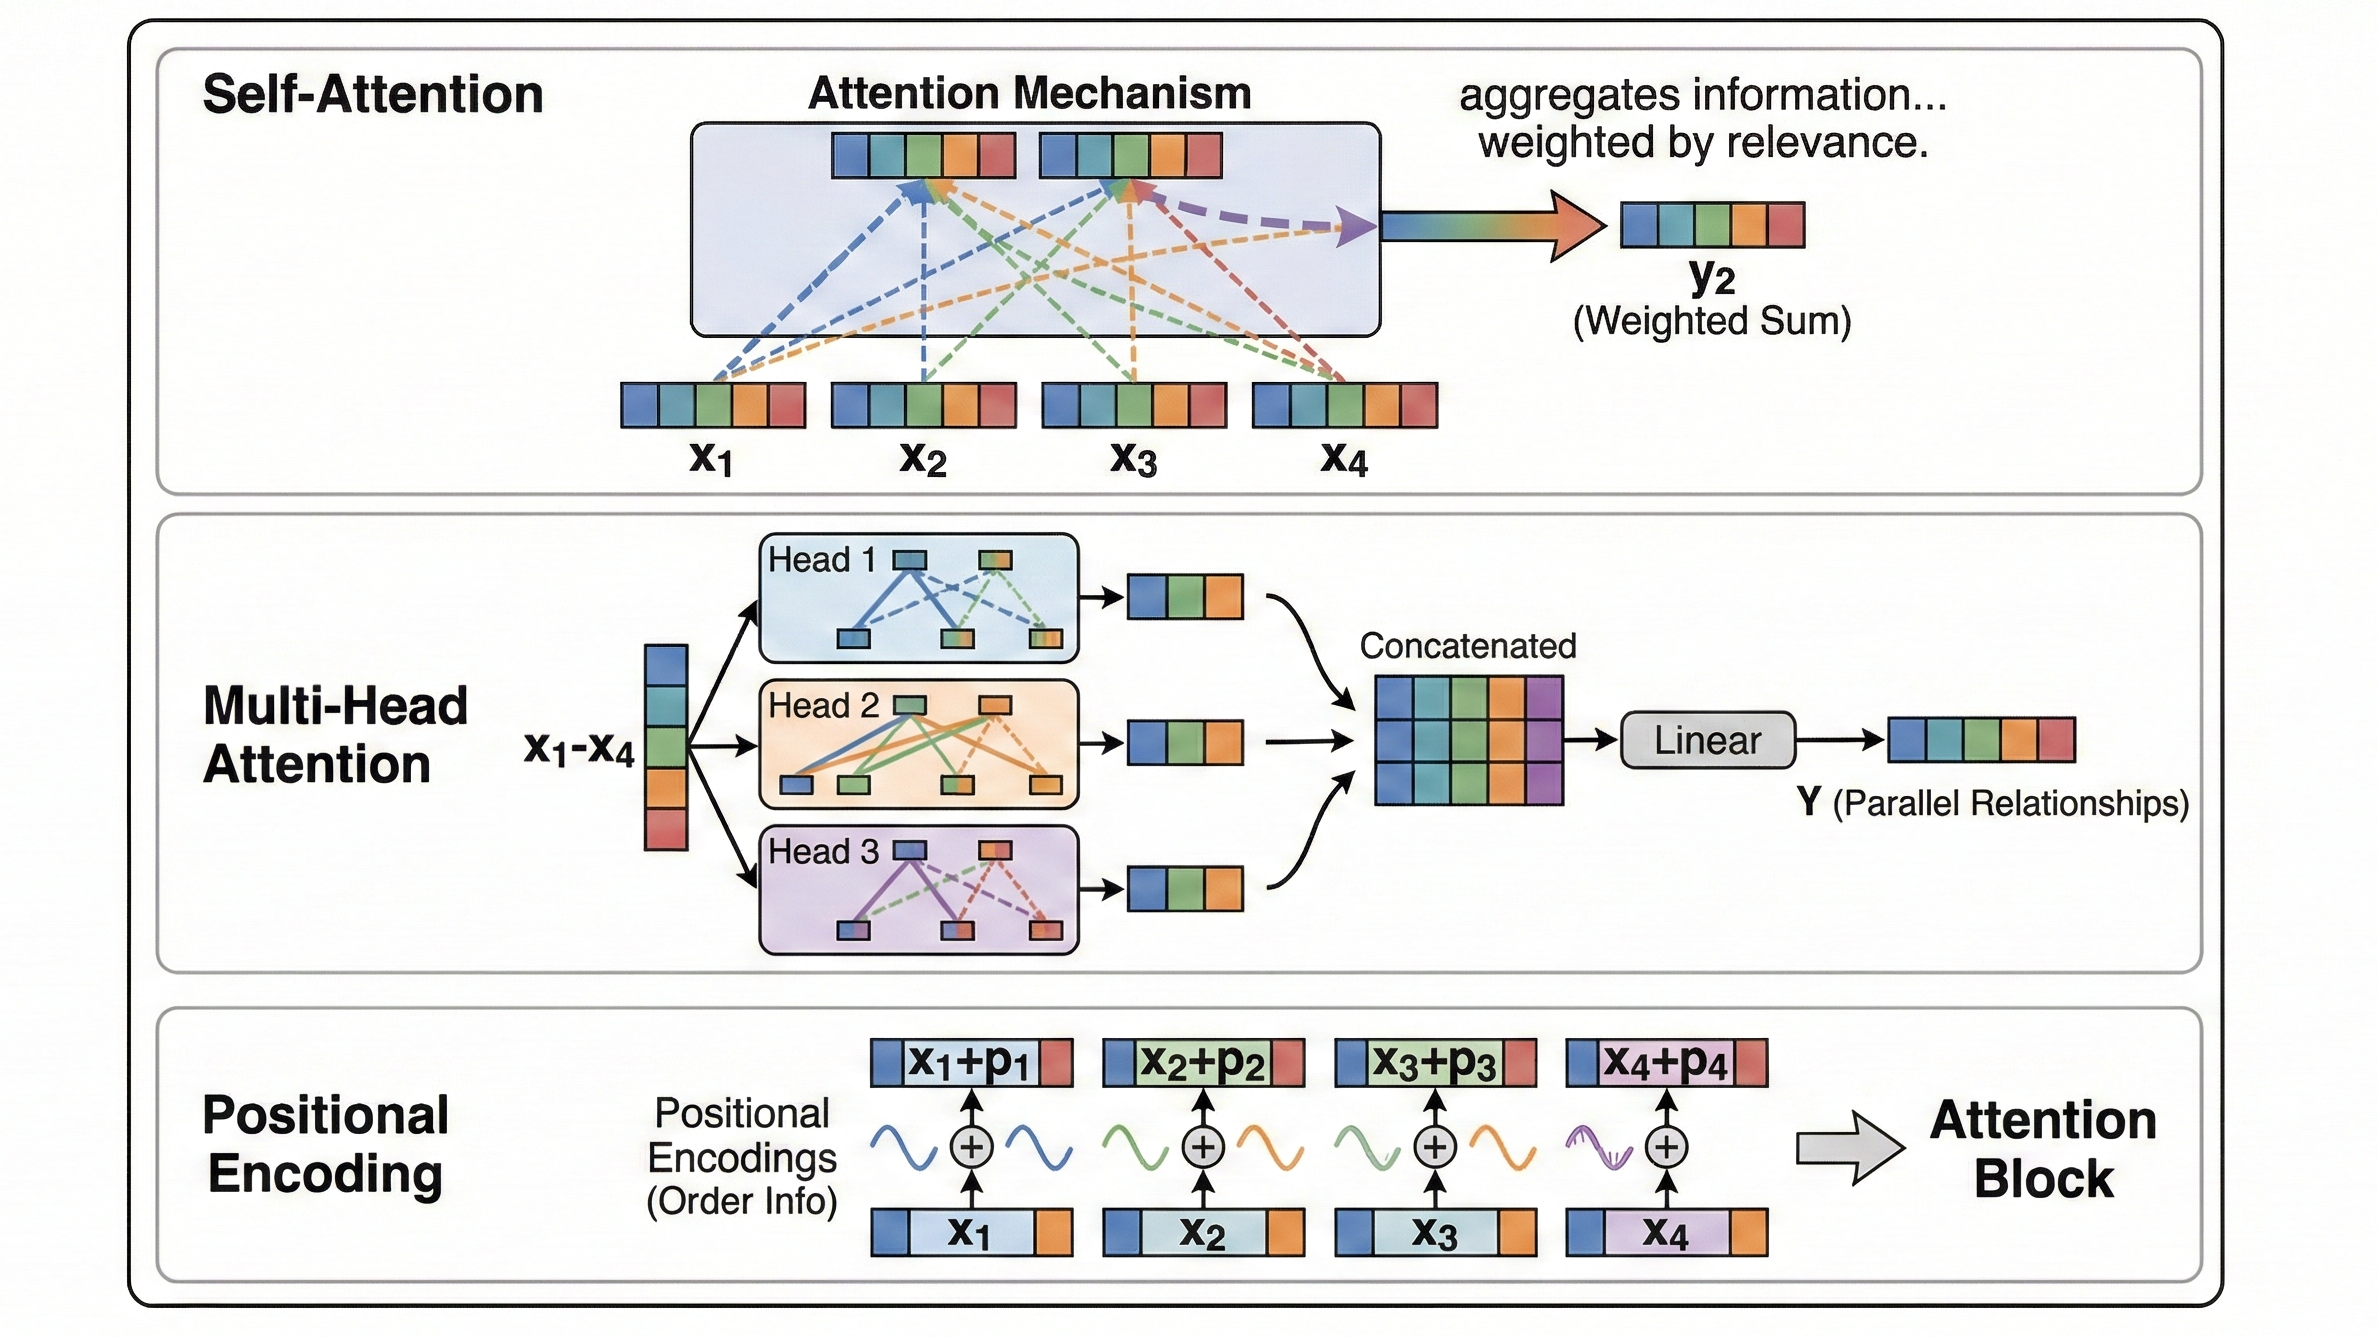
\includegraphics[width=0.9\textwidth]{figures/fig-transformer-attention}
\caption{缩放点积注意力(scaled dot-product attention)的计算流程:由输入生成查询 $Q$、键 $K$、值 $V$,计算相似度并缩放,经 softmax 得到注意力权重,再用权重对 $V$ 做加权求和得到输出。}
\label{fig:transformer-attention}
\end{figure}
\medskip

\noindent 图~\ref{fig:transformer-attention}~展示的并不是完整 Transformer 的所有组件,而是其最核心、最基础的运算单元:缩放点积注意力。图中左侧给出三类输入张量:查询(Query, $Q$)、键(Key, $K$)和值(Value, $V$)。注意力的第一步是用查询去"匹配"键:对每个查询向量与所有键向量计算点积相似度,并按维度做缩放(Dot Product \& Scaling),得到相关性分数矩阵;第二步用 softmax 将分数归一化为注意力权重(Attention Weights),图中以热力图形式呈现,表示"每个查询位置对各键位置分配了多少关注";第三步用这些权重对值向量做加权求和(Weighted Sum),得到输出(Output)。因此,注意力的本质可以概括为:用 $Q$ 与 $K$ 计算"该看哪里",再用该权重对 $V$ 汇聚"要拿什么信息",从而实现跨位置的信息融合。

\noindent Transformer 与循环网络、卷积网络的本质区别,在于信息交互的路径。循环网络的信息需要沿时间步逐步传递,长距离依赖往往意味着长路径;卷积网络的信息主要在局部邻域内传播,想"看到"很远的位置通常需要堆叠很多层以扩大感受野。Transformer 通过注意力机制让任意两个位置在一次计算中直接交互,从而把"全局依赖"变成一次可并行的矩阵运算。设输入序列长度为 $n$,每个位置的表示维度为 $d$,把输入堆叠成矩阵 $X\in\mathbb R^{n\times d}$,其中第 $i$ 行 $x_i^\top$ 表示第 $i$ 个 token 的向量表示;token 可以是词、子词、帧或图像 patch 等基本单元。注意力的核心思想是:对每个位置 $i$,模型会在所有位置 $j$ 上分配权重,再把各位置的表示按权重加权求和,从而得到位置 $i$ 的新表示;可以把它理解为"位置 $i$ 在更新自己的表示时,会去全序列范围内借信息,但借多少由相关性决定"。

\noindent 在计算上,Transformer 先把同一个输入 $X$ 通过三组线性映射生成查询、键、值:
\[ Q=XW_Q,\qquad K=XW_K,\qquad V=XW_V,\]
其中 $W_Q,W_K,W_V\in\mathbb R^{d\times d_k}$,因此 $Q,K,V\in\mathbb R^{n\times d_k}$。直观地看,$q_i$ 表示位置 $i$"需要什么信息"的查询表达,$k_j$ 表示位置 $j$"具有什么信息特征"的标识,$v_j$ 则是位置 $j$ 实际可被汇聚的内容。然后对任意两个位置 $i,j$,以点积 $q_i^\top k_j$ 衡量相关性,并做缩放与 softmax 归一化得到注意力权重矩阵
\[ A=\mathrm{softmax}\!\left(\frac{QK^\top}{\sqrt{d_k}}\right),\qquad A\in\mathbb R^{n\times n},\]
其中 $A_{i,j}$ 表示在更新位置 $i$ 的表示时对位置 $j$ 的关注程度;最后用这些权重对 $V$ 做加权汇总:
\[ \mathrm{Attn}(X)=AV,\qquad \mathrm{Attn}(X)\in\mathbb R^{n\times d_k}.\]
图~\ref{fig:transformer-attention}~中"Dot Product \& Scaling $\rightarrow$ Softmax $\rightarrow$ Attention Weights $\rightarrow$ Weighted Sum"的流程正对应上述公式:缩放点积给出相关性分数,softmax 把分数转成可解释的权重分布,随后对 $V$ 的加权求和产生输出。由于权重是对所有位置分配的,注意力不是"选一个位置",而是"以分布的形式融合多处信息",因此它既能表达局部依赖,也能表达长距离依赖。

\noindent 但序列中的相关性往往不止一种,仅用一套相似度空间去衡量所有关系会受到表达瓶颈限制。以语言为例,相关性可能来自语义相近、语法依赖、指代关系或主题一致等不同维度;以视觉 patch 序列为例,相关性可能来自局部纹理相似、同一物体的不同部位、或跨区域的形状对应。实际 Transformer 通常采用多头注意力:把图~\ref{fig:transformer-attention}~所示的注意力机制并行复制为 $h$ 个头,每个头拥有独立的线性投影,从而在不同子空间中学习不同的关注模式。设第 $t$ 个头计算
\[ \mathrm{head}_t=\mathrm{Attn}(XW_Q^{(t)},XW_K^{(t)},XW_V^{(t)}),\]
再把各头输出拼接并线性融合:
\[ \mathrm{MHA}(X)=\mathrm{Concat}(\mathrm{head}_1,\dots,\mathrm{head}_h)\,W_O.\]
多头机制的价值在于把复杂关系分摊到并行的子空间中表达,而不是强迫所有关系挤进同一种相似度度量里:有的头可能更偏向近邻交互,有的头可能更善于捕捉长距离依赖;有的头可能对某类结构模式(如语法骨架、物体轮廓)更敏感。

\noindent 注意力机制本身只依赖向量间的相似度,它并不天然携带"第几个位置"的信息。若只看 $QK^\top$ 的计算形式,序列顺序的变化不会通过任何显式项被编码进相似度评分中,这会导致模型难以区分"同样的 token 出现在不同位置"所对应的不同语义。对语言与时间序列而言,这是一个根本问题:词序变了,含义往往就变了;时间戳的位置不同,事件的意义也不同。因此 Transformer 需要显式地把位置信息注入输入表示,最常见的做法是位置编码。设 $P\in\mathbb R^{n\times d}$ 为位置向量矩阵,将其与输入相加:
\[ X' = X + P.\]
这样模型在后续生成 $Q,K,V$ 时就同时包含内容信息与位置信息。位置编码可以是固定的函数形式(如正弦余弦),也可以是可学习参数;无论采用哪种方案,其目的都是让模型具备对顺序的可辨识性,否则注意力只能表达"哪些内容相似",却难以表达"这些内容以何种顺序组织"。

\noindent 将上述机制组织为可堆叠、可训练的网络模块后,得到 Transformer 的基本层结构。常用的基本块由两部分组成:注意力子层与前馈网络(FFN)子层。前馈网络对每个位置独立地做两层线性变换与非线性:
\[ \mathrm{FFN}(x)=W_2\,\phi(W_1x+b_1)+b_2,\]
它的作用是对每个位置的表示进行非线性加工,并通过中间维度的扩展与压缩增强表达能力。注意力负责在不同位置之间交换与融合信息,前馈网络负责对每个位置内部的表示做更强的非线性变换;两者交替堆叠,就形成了 Transformer 的深层表示学习。为了让深层堆叠保持可训练与数值稳定,Transformer 通常配合残差连接与归一化(LayerNorm)。一种常见写法是
\[ H_1 = \mathrm{LN}(X + \mathrm{MHA}(X)),\qquad H_2 = \mathrm{LN}(H_1 + \mathrm{FFN}(H_1)).\]
可以把它理解为:图~\ref{fig:transformer-attention}~所示的注意力计算负责"跨位置聚合信息",前馈网络负责"在位置内做非线性加工",残差连接确保信息与梯度能够顺畅流动,归一化缓解数值尺度漂移,从而使多层堆叠在优化上可行。

\noindent 为了把注意力从公式落到可计算的步骤上,可以用一个极简数值示例展示"相关性—权重—加权汇总"的流程。考虑三个 token 的某一头的 $Q,K,V$(为便于手算,向量维度取 $2$):
\[ q_1=(1,0),\ q_2=(0,1),\ q_3=(1,1),\qquad k_1=(1,0),\ k_2=(0,1),\ k_3=(1,1),\qquad v_1=(1,0),\ v_2=(0,1),\ v_3=(1,1).\]
以位置 $3$ 为例,其对三个位置的未归一化相关性(点积)为
\[ q_3^\top k_1=1,\qquad q_3^\top k_2=1,\qquad q_3^\top k_3=2.\]
softmax 会把这些分数映射为非负且和为 $1$ 的权重,因而位置 $3$ 会对自身分配更大的权重,同时也会对位置 $1$ 与位置 $2$ 分配一定权重。最终位置 $3$ 的输出是
\[ o_3=\sum_{j=1}^3 a_{3j} v_j,\]
即对三处的值向量按权重加权融合。这个例子强调的要点是:注意力把"应该向哪些位置借信息、借多少"具体化为一组可学习的权重分布,使得每个位置在一次计算中就能获得全局上下文;多头机制则让这种信息聚合同时具备多种并行视角,而位置编码保证这种融合不会丢失顺序结构。理解这些机制后,读者再去学习更具体的 Transformer 变体(如编码器/解码器结构、掩码注意力、交叉注意力、长序列改进等)时,会更清楚每一处改动究竟在改变信息如何流动,以及相应改变了哪些计算代价与归纳偏置。
